\chapter{Avaliação do método proposto}
\label{chap:avaliacao}
% http://www.ppgia.pucpr.br/~fabricio/ftp/Aulas/Mestrado/IA/Nievola/MD/MD-06-Agrupamento.pdf
Para a avaliação do método proposto diferentes aspectos de validação de grupos são analisados, como:
\begin{itemize}
    \item Comparar os resultados de uma análise de grupos com resultados conhecidos;
    \item Indicar se uma estrutura não aleatória realmente existe num conjunto de dados;
    \item Comparar os resultados de dois diferentes conjuntos de análise de grupos para determinar qual deles é melhor;
    \item Determinar o número de grupos.
\end{itemize}

Para validar a saída gerada pelo processo de agrupamento, recorre-se a critérios de otimalidade pré-estabelecidos, com as seguintes características:
\begin{itemize}
    \item o problema possui um conjunto de variáveis manipuláveis no procedimento de busca pelo ótimo, que são as variáveis de decisão do problema;
    \item os valores assumidos pelas variáveis de decisão devem satisfazer um conjunto de restrições, que compõe a região de soluções viáveis do problema;
    \item as variáveis de decisão do problema podem assumir valores pré-estabelecidos.
\end{itemize}

\section{Testes de Predição e análise}

Foram implementados gráficos de séries temporais que são usados para examinar as variações semanais de uma mudança epidemiológica. Com essas métricas, pode-se comparar padrões de dados, como o número total de casos de Dengue de uma determinada semana com o número de casos dentro de algum grupo de previsão, definido pelo método proposto com base nas semanas anteriores a semana em análise.


\section{Testes de comparação de predições baseado nos grupos anteriores}

As figuras a seguir apresentam gráficos sobre dengue e chikungunya, nos anos de 2017 e 2018, levando em consideração as 4 semanas anteriores a semana do grupo de previsão, a variável Eps do ST-DBSCAN de 500 metros e pelo menos 1 caso para caracterizar um grupo.
As legendas indicam três tipos:
\begin{itemize}
    \item Número de casos dentro de algum grupo de previsão, representado pela cor verde;
    \item Número de casos fora de algum grupo de previsão, representado pela cor azul;
    \item Número total de casos, representado pela cor laranja.
\end{itemize}

A figura \ref{fig:metricasDengue201745001} apresenta uma grande quantidade de casos dentro de algum grupo de previsão ao longo do ano.
\begin{figure}[!ht]
	\centering	
	\Caption{\label{fig:metricasDengue201745001} Métricas: Dengue/2017, 4 semanas, Eps 500m, MinPts 1}
	\UECEfig{}{
		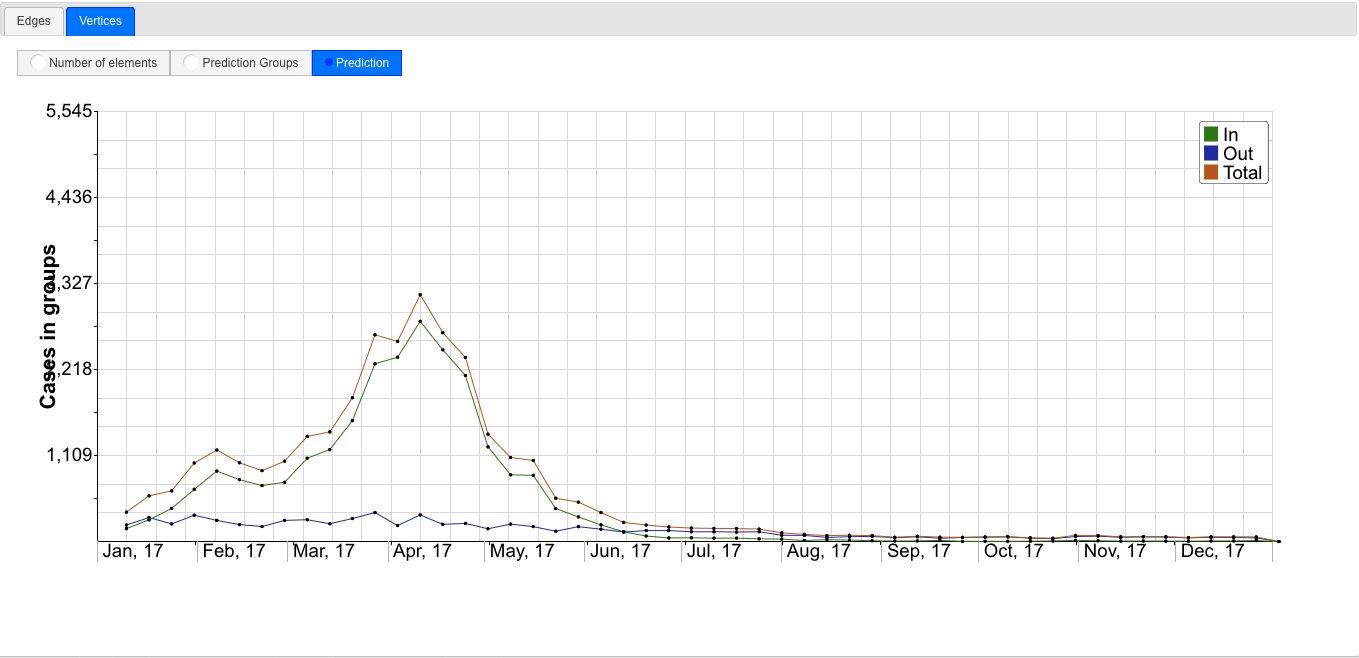
\includegraphics[width=15cm]{figuras/metricas/DENGUE_2017_4_500_1.png}
	}{
		\Fonte{Elaborado pelo autor}
	}
\end{figure}
\FloatBarrier

A figura \ref{fig:agrupamentosDengue2017} representa a seguinte análise:
\begin{itemize}
    \item Análise dos casos de Dengue em 2017;
    \item Semana 18 do ano em análise;
    \item Semanas  14, 15, 16 e 17 analisadas para gerar os grupos de previsão da semana 18;
    \item 252 grupos de predição gerados;
    \item 208 grupos com pelo menos um caso dentro;
    \item 1384 casos de Dengue na semana em análise;
    \item 1220 casos dentro de algum grupo de previsão;
    \item 164 casos fora dos grupos de previsão.
\end{itemize}

Podemos observar que o número de casos dentro de algum grupo de previsão é alto devido a proximidade entre os grupos, sendo assim, abrangendo uma grande área com possíveis casos.

\begin{figure}[!ht]
	\centering
	\Caption{\label{fig:agrupamentosDengue2017} Agrupamentos: Dengue/2017}
	\UECEfig{}{
		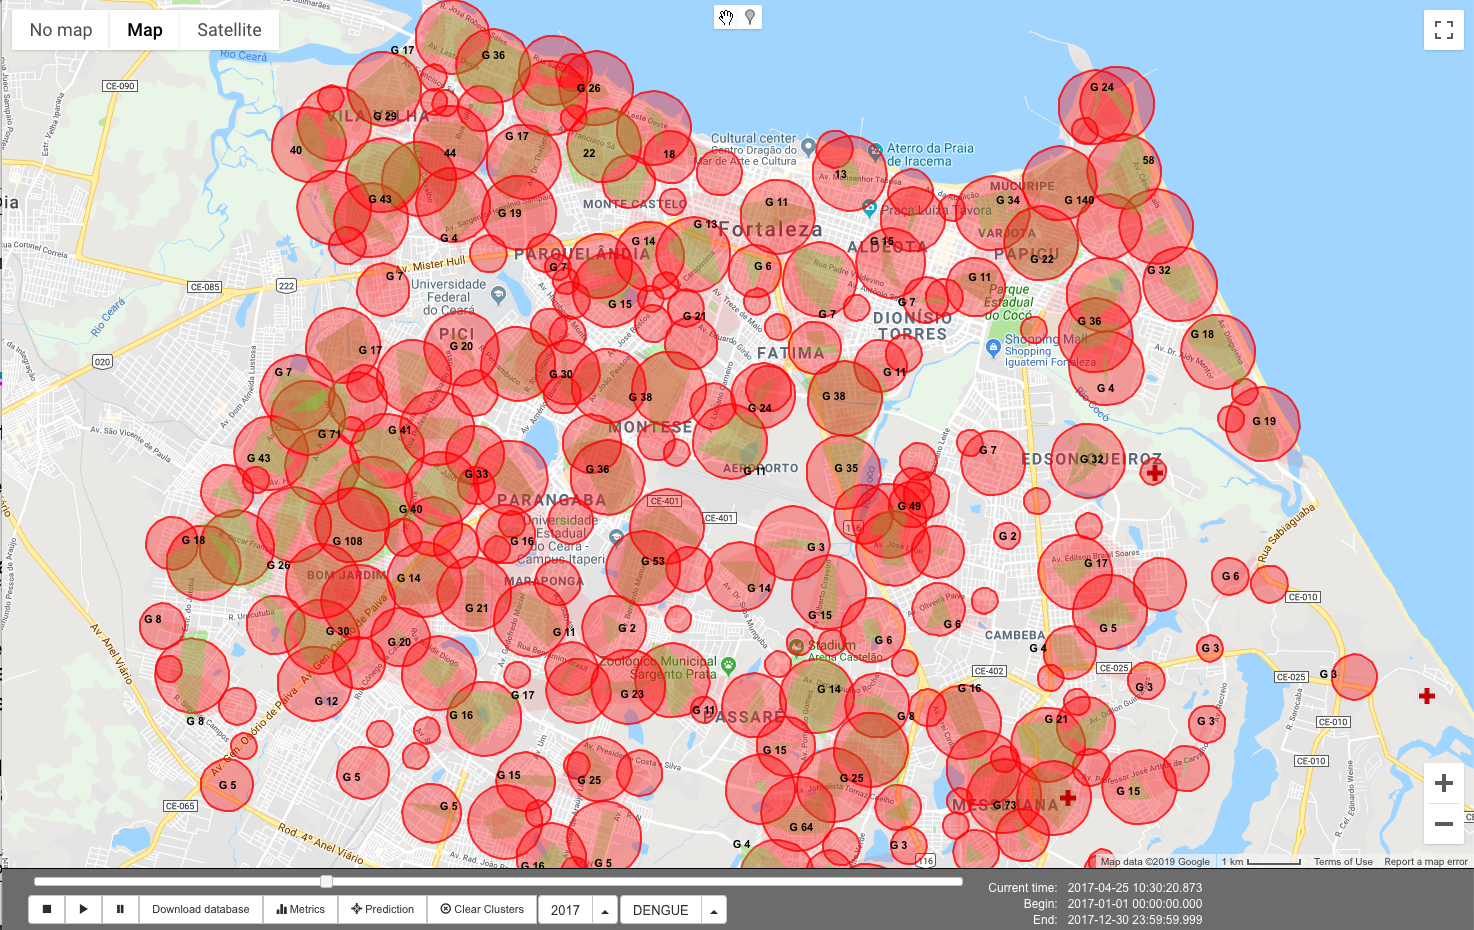
\includegraphics[width=15cm]{figuras/predicao/dengue2017Week17.png}
	}{
		\Fonte{Elaborado pelo autor}
	}
\end{figure}
\FloatBarrier

O cálculo do raio dos grupos de previsão apresentados é dado por:
${\sqrt[]{p} * 250, p \leqslant 8}$, onde ${p}$ é o número de casos previstos por grupo de previsão gerado pelo ST-DBSCAN. Logo, o raio máximo dos grupos de previsão da figura \ref{fig:agrupamentosDengue2017} é aproximadamente 700m.

A figura \ref{fig:metricasDengue201845001} apresenta o número de casos fora de algum grupo de previsão maior que dentro de algum grupo de previsão, praticamente em todas as semanas analisadas.
\begin{figure}[!ht]
	\centering	
	\Caption{\label{fig:metricasDengue201845001} Métricas: Dengue/2018, 4 semanas, Eps 500m, MinPts 1}
	\UECEfig{}{
		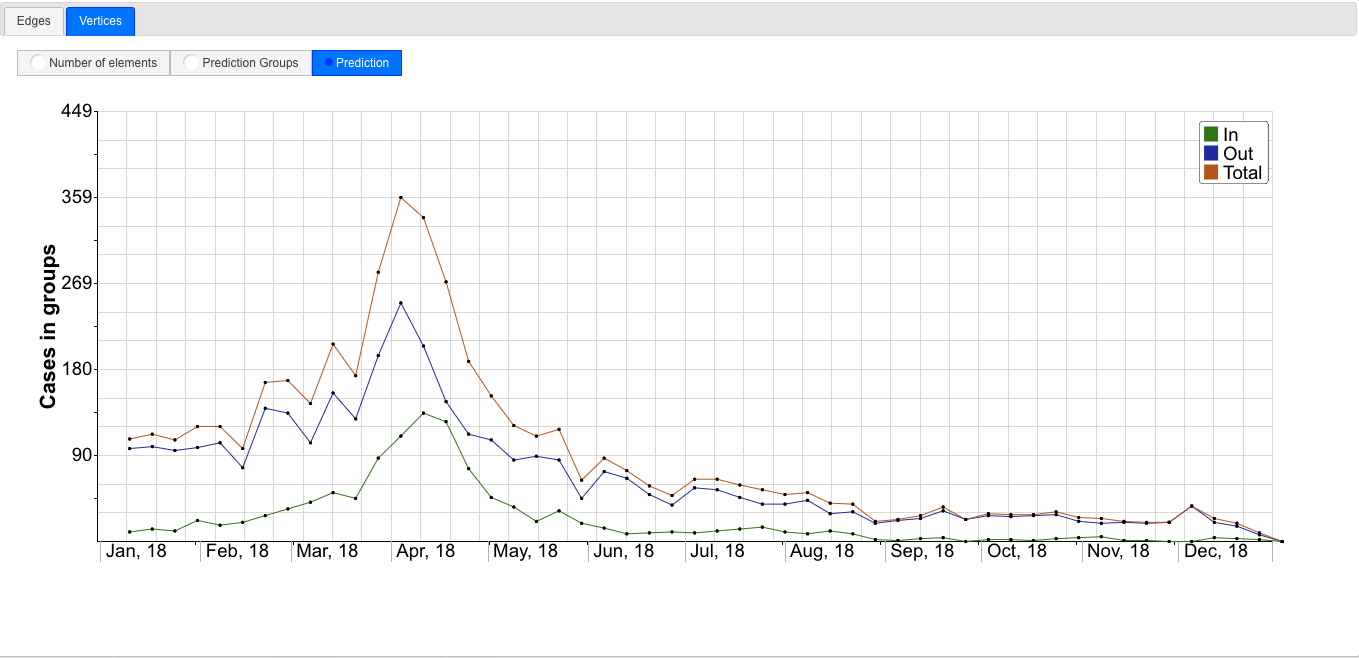
\includegraphics[width=15cm]{figuras/metricas/DENGUE_2018_4_500_1.png}
	}{
		\Fonte{Elaborado pelo autor}
	}
\end{figure}
\FloatBarrier

Observa-se na figura \ref{fig:metricasChi201745001} semelhança ao gráfico da figura \ref{fig:metricasDengue201745001}, onde dada a grande quantidade de casos de endemia dentro de uma pequena região, os grupos de previsão conseguem abranger uma grande área com possiveis casos.
\begin{figure}[!ht]
	\centering	
	\Caption{\label{fig:metricasChi201745001} Métricas: Chikungunya/2017, 4 semanas, Eps 500m, MinPts 1}
	\UECEfig{}{
		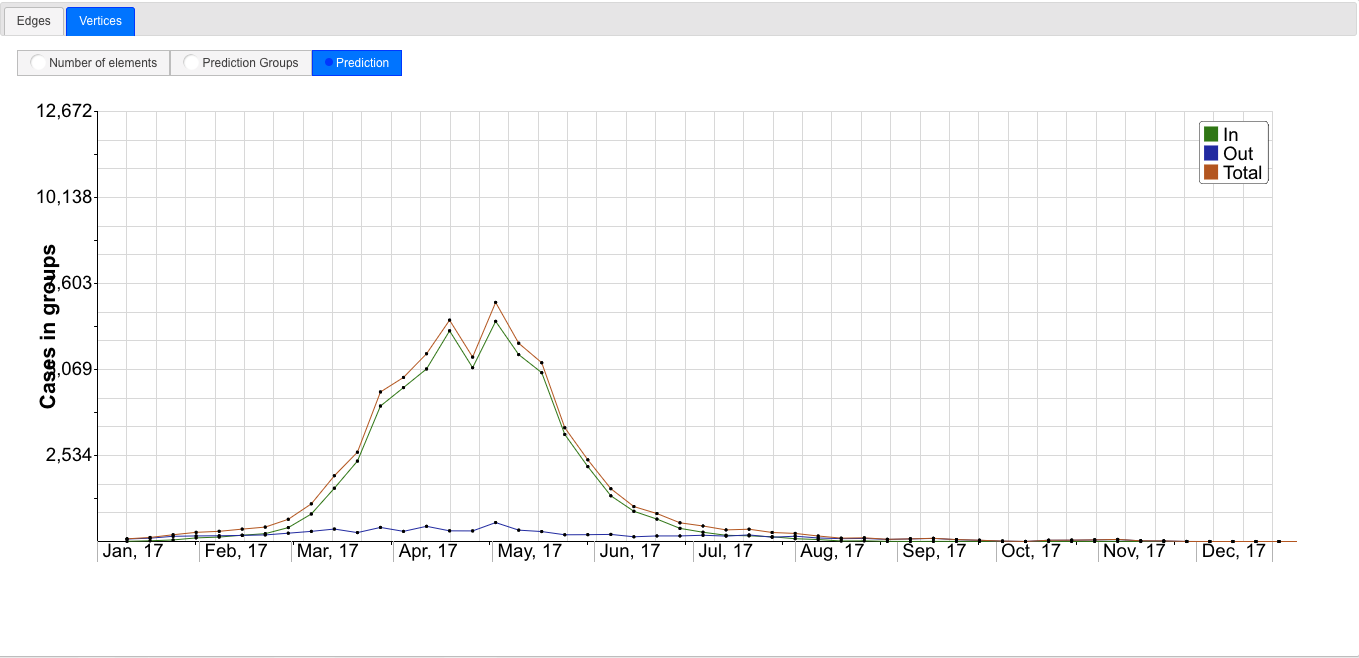
\includegraphics[width=15cm]{figuras/metricas/CHI_2017_4_500_1.png}
	}{
		\Fonte{Elaborado pelo autor}
	}
\end{figure}
\FloatBarrier

Dado o número baixo de casos de Chikungunya em 2018 em Fortaleza-CE, somente alguns grupos de previsão conseguiram gerar dados não-nulos, como mostra o gráfico da figura \ref{fig:metricasChi201845001}.
\begin{figure}[!ht]
	\centering	
	\Caption{\label{fig:metricasChi201845001} Métricas: Chikungunya/2018, 4 semanas, Eps 500m, MinPts 1}
	\UECEfig{}{
		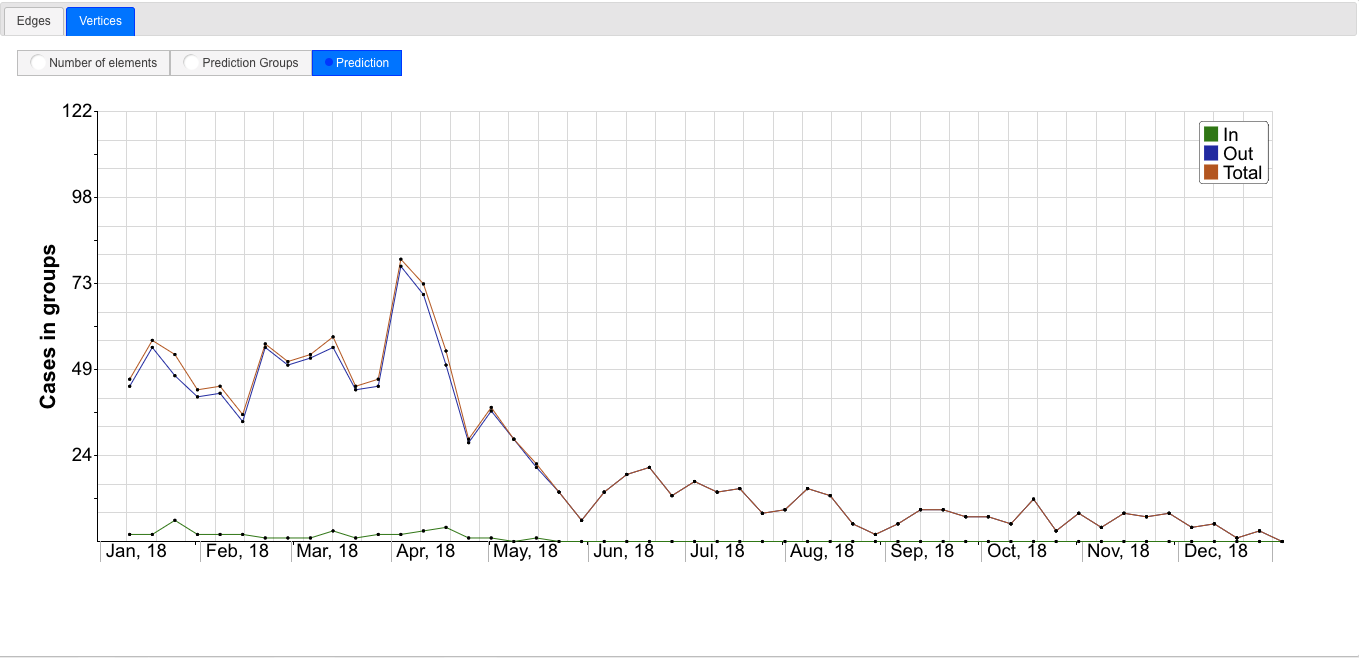
\includegraphics[width=15cm]{figuras/metricas/CHI_2018_4_500_1.png}
	}{
		\Fonte{Elaborado pelo autor}
	}
\end{figure}
\FloatBarrier


Outra forma de exibir os resultados das figuras anteriores na forma de gráfico de colunas empilhadas são dadas em \ref{ap:graphicColBar}
